\chapter{Explanation of \textbf{MAIN.ipynb} file}\label{ch:explanation-of-main-file}

This is a short explanation about the Jupiter Notebook \emph{MAIN.ipynb} in the root directory of the project's repository.
The Notebook aggregates and condenses all functionalities of the Python code.

\begin{figure}[H]   %[h] puts picture right here. 't' stands for to, 'b' stands for bottom
    \centering
    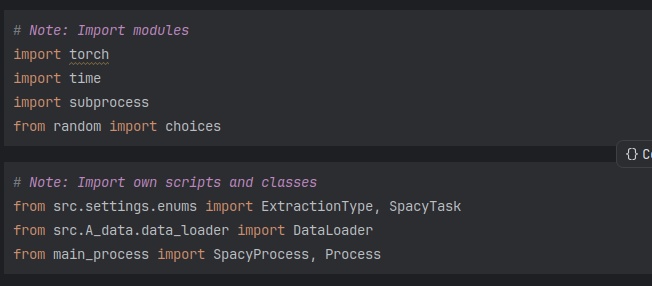
\includegraphics[width=0.95\textwidth]{Assets/main-1}
    \caption{STEP 1: Import libraries}
    \label{fig:main-1}
\end{figure}

\begin{figure}[H]   %[h] puts picture right here. 't' stands for to, 'b' stands for bottom
    \centering
    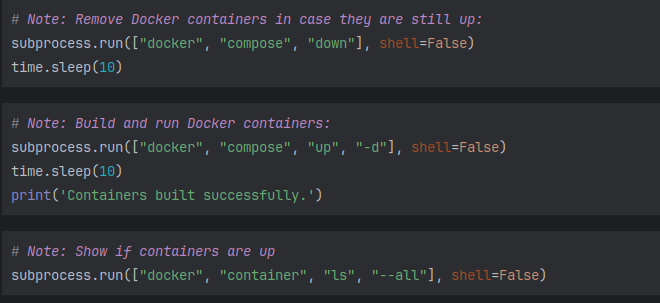
\includegraphics[width=0.95\textwidth]{Assets/main-2}
    \caption{STEP 2: Start Docker container}
    \label{fig:main-2}
\end{figure}
\begin{figure}[H]   %[h] puts picture right here. 't' stands for to, 'b' stands for bottom
    \centering
    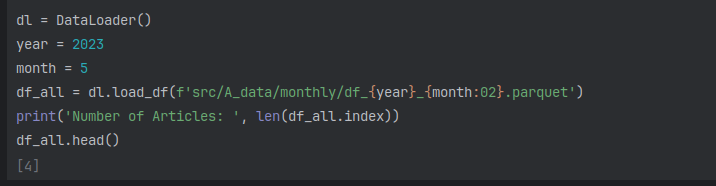
\includegraphics[width=0.95\textwidth]{Assets/main-3}
    \caption{STEP 3: Load News Articles}
    \label{fig:main-3}
\end{figure}
\begin{figure}[H]   %[h] puts picture right here. 't' stands for to, 'b' stands for bottom
    \centering
    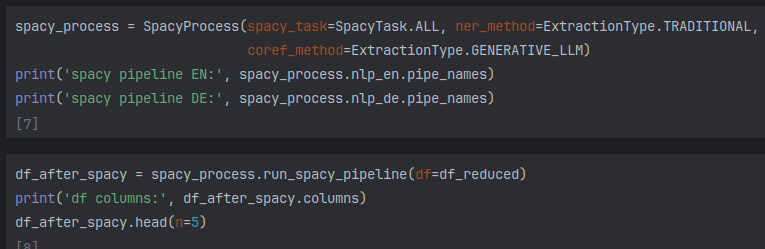
\includegraphics[width=0.95\textwidth]{Assets/main-4}
    \caption{STEP 4: Run spacy pipeline (NER, COREF)}
    \label{fig:main-4}
\end{figure}
\begin{figure}[H]   %[h] puts picture right here. 't' stands for to, 'b' stands for bottom
    \centering
    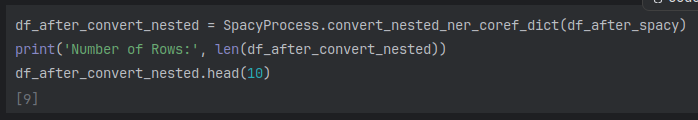
\includegraphics[width=0.95\textwidth]{Assets/main-5}
    \caption{STEP 5: Convert Nested Dictionary}
    \label{fig:main-5}
\end{figure}
\begin{figure}[H]   %[h] puts picture right here. 't' stands for to, 'b' stands for bottom
    \centering
    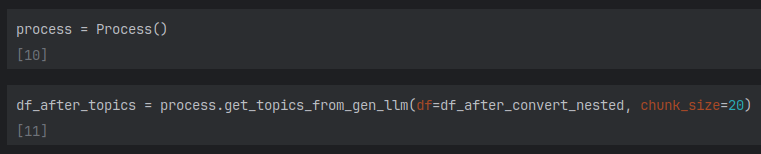
\includegraphics[width=0.95\textwidth]{Assets/main-6}
    \caption{STEP 6: Start Topic Modelling Process}
    \label{fig:main-6}
\end{figure}
\begin{figure}[H]   %[h] puts picture right here. 't' stands for to, 'b' stands for bottom
    \centering
    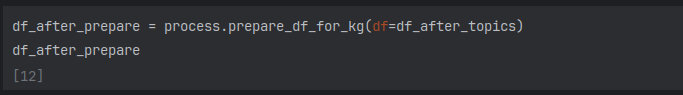
\includegraphics[width=0.95\textwidth]{Assets/main-7}
    \caption{STEP 7: Prepare DataFrame for Knowledge Graph}
    \label{fig:main-7}
\end{figure}
\begin{figure}[H]   %[h] puts picture right here. 't' stands for to, 'b' stands for bottom
    \centering
    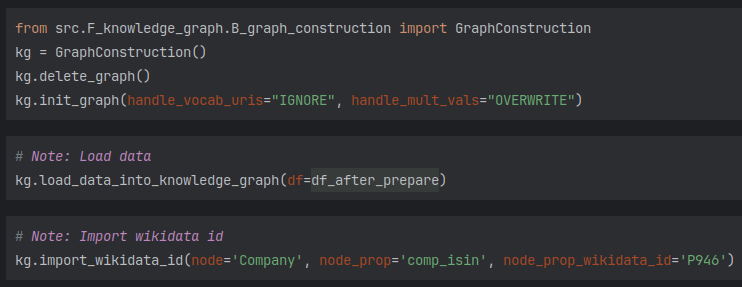
\includegraphics[width=0.95\textwidth]{Assets/main-8}
    \caption{STEP 8: Initialize Knowledge Graph and load Data}
    \label{fig:main-8}
\end{figure}
\begin{figure}[H]   %[h] puts picture right here. 't' stands for to, 'b' stands for bottom
    \centering
    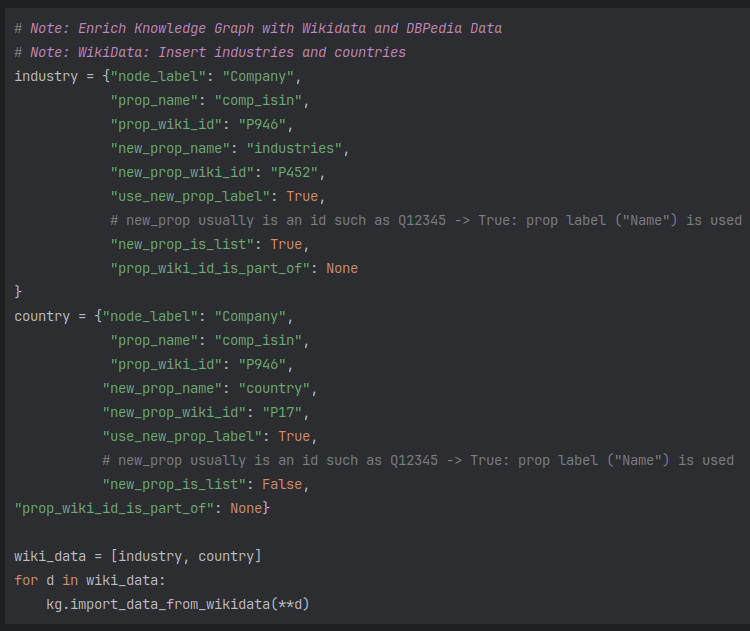
\includegraphics[width=0.95\textwidth]{Assets/main-9}
    \caption{STEP 9: Enrich Knowledge Graph with Data from Wikidata}
    \label{fig:main-9}
\end{figure}
\begin{figure}[H]   %[h] puts picture right here. 't' stands for to, 'b' stands for bottom
    \centering
    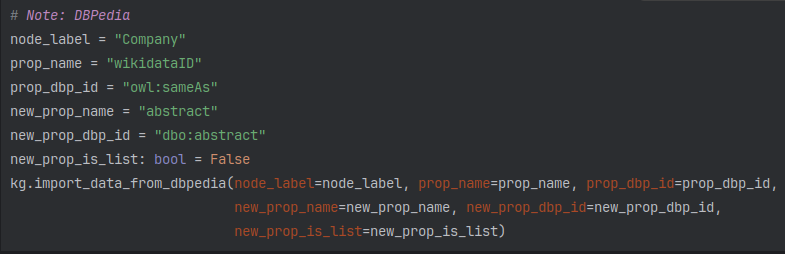
\includegraphics[width=0.95\textwidth]{Assets/main-10}
    \caption{STEP 10: Enrich Knowledge Graph with Data from DBPedia}
    \label{fig:main-10}
\end{figure}
\begin{figure}[H]   %[h] puts picture right here. 't' stands for to, 'b' stands for bottom
    \centering
    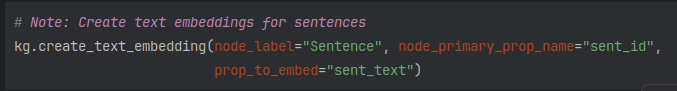
\includegraphics[width=0.95\textwidth]{Assets/main-11}
    \caption{STEP 11: Create Sentence Text Embeddings}
    \label{fig:main-11}
\end{figure}
\begin{figure}[H]   %[h] puts picture right here. 't' stands for to, 'b' stands for bottom
    \centering
    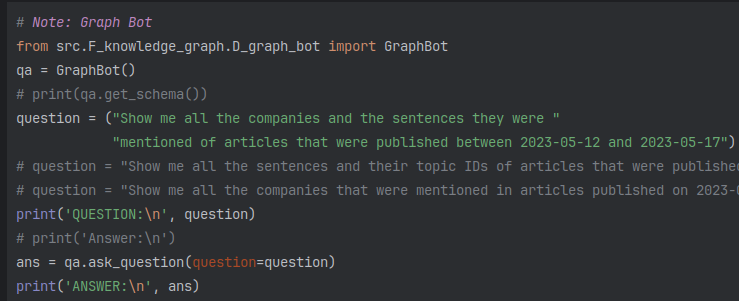
\includegraphics[width=0.95\textwidth]{Assets/main-12}
    \caption{STEP 12: Communicate with Graph Bot}
    \label{fig:main-12}
\end{figure}
